\chapter{Prosperity Manual Trading Challenges}
\label{ch:manual_rounds}
\chaptermark{Manual trading challenges}

Manual rounds test trading intuition without code: game theory,
probability, and quick mental arithmetic rather than Python.  Every
Prosperity competition pairs each algorithmic round with a manual
challenge solved by hand.  Manual PnL is a modest slice of the total,
but the skills transfer directly to a trading floor, where a junior
trader who cannot do fast expected-value calculations in their head
is a liability.

This chapter catalogues the five recurring archetypes from
Prosperity~1--3, each treated with the mathematics it deserves:
\begin{enumerate}
  \item FX triangular arbitrage (brute-force optimisation under
  time pressure).
  \item Container auctions (expected value under uncertainty,
  winner's curse).
  \item Reserve-price / valuation rounds (microstructure as game,
  bid--ask positioning).
  \item Suitcase / Nash bargaining (cooperative game theory,
  surplus division).
  \item News trading (Bayesian updating, position sizing under
  signal noise).
\end{enumerate}

\begin{backgroundbox}[Prerequisites]
\begin{itemize}
  \item \Cref{ch:arbitrage_zoo}, \S\ref{sec:ch13_triangular}:
  triangular FX arbitrage --- computing round-trip products,
  trading when the product exceeds one.
  \item \Cref{ch:kelly_risk}: the Kelly criterion and
  expected-value-based position sizing.
  \item \Cref{ch:kyle_gm}: Glosten--Milgrom Bayesian updating
  of a market maker's belief about the true value of an asset.
  \item Basic probability: Bayes' theorem, expected value,
  conditional expectation. \Cref{ch:price_value} covers these
  in the trading context.
  \item No game theory is assumed; this chapter introduces the
  required concepts (Nash equilibrium, Nash bargaining solution,
  winner's curse) from scratch.
\end{itemize}
\end{backgroundbox}

%======================================================================
\section{FX triangular arbitrage}
\label{sec:ch25_fx_arb}
%======================================================================

The simplest manual round is a currency conversion puzzle.  Given
an $n \times n$ conversion matrix~$\mathbf{M}$ (entry $M_{ij}$ is
the units of currency~$j$ received per unit of~$i$ sold), find a
sequence of at most~$k$ trades (typically $k = 5$) that maximises
the final amount of your starting currency.

\subsection{Mathematical framework}

The matrix defines a directed weighted graph $G = (V, E, w)$:
currencies are vertices, conversions are edges, weights are rates.
A $k$-trade sequence is a walk of length~$k$ starting and ending
at the source currency, with final amount equal to the edge-weight
product:
\begin{equation}
  \text{return}
  \;=\;
  \prod_{t=1}^{k} M_{c_{t-1},\, c_t}
  \label{eq:ch25_fx_return}
\end{equation}
with $c_0 = c_k$ the starting currency.  Profitable iff
$\text{return} > 1$.  Find the length-$\le k$ walk maximising
the product.

\begin{keyfactbox}[Triangular arbitrage indicator]
For a three-currency cycle $A \to B \to C \to A$, the profit
per unit is
\[
  \Delta \;=\;
  M_{A,B} \cdot M_{B,C} \cdot M_{C,A} - 1.
\]
If $\Delta > 0$, the cycle is profitable.  This is the same
triangular arbitrage indicator derived in
\cref{sec:ch13_triangular}.
\end{keyfactbox}

\subsection{Worked example: Prosperity~3, Round~1}

Prosperity~3 Round~1 provided a $4 \times 4$ conversion matrix
between four in-game currencies \citep{frankfurtHedgehogs2025imcP3}:

\medskip
\begin{center}
\begin{tabular}{l c c c c}
\toprule
 & \textbf{Snowballs} & \textbf{Pizza} & \textbf{Si.\ Nuggets} & \textbf{SeaShells} \\
\midrule
\textbf{Snowballs}      & 1.00 & 1.45 & 0.52 & 0.72 \\
\textbf{Pizza}           & 0.70 & 1.00 & 0.31 & 0.48 \\
\textbf{Si.\ Nuggets}    & 1.95 & 3.10 & 1.00 & 1.49 \\
\textbf{SeaShells}       & 1.34 & 1.98 & 0.64 & 1.00 \\
\bottomrule
\end{tabular}
\end{center}
\medskip

Starting from SeaShells with five trades, the Frankfurt Hedgehogs
enumerated all paths.  The optimum:
\[
  \texttt{SeaShells}
  \xrightarrow{1.34}
  \texttt{Snowballs}
  \xrightarrow{0.52}
  \texttt{Si.\ Nuggets}
  \xrightarrow{3.10}
  \texttt{Pizza}
  \xrightarrow{0.70}
  \texttt{Snowballs}
  \xrightarrow{0.72}
  \texttt{SeaShells}
\]
Product of rates:
\[
  1.34 \times 0.52 \times 3.10 \times 0.70 \times 0.72
  \;=\;
  \underbrace{1.34 \times 0.52}_{0.6968}
  \;\times\;
  \underbrace{3.10 \times 0.70}_{2.17}
  \;\times\; 0.72
  \;\approx\; 1.089
\]
yielding approximately $8.9\%$ profit per round trip.

\subsection{Connection to graph theory}

The general problem---maximum-weight walk of length~$\le k$---is
solved by Bellman--Ford in log-space: set $w'_{ij} = -\ln M_{ij}$,
then the rate product equals $\exp(-\sum w'_{ij})$, so maximising
the product is equivalent to finding a minimum-weight walk (a
negative-total-weight walk is a profitable round trip).  Real-world
FX desks run this continuously on live quotes \citeBouchaud.

For the competition, brute force suffices: $n = 4$, $k = 5$ gives
$4^5 = 1{,}024$ walks---minutes by hand.

\subsection{Manual skill: speed under time pressure}

Under time pressure on a $4 \times 4$ matrix:
\begin{enumerate}
  \item \textbf{Eliminate dominated currencies}---drop any row
  uniformly worse than another.
  \item \textbf{Check all three-cycles first}: at most
  $\binom{4}{3} \times 2 = 8$ oriented three-cycles.
  \item \textbf{Extend promising three-cycles to five-step paths.}
  If $A \to B \to C \to A$ has $\Delta > 0$, try splitting one
  leg into two intermediate conversions that beat the direct rate.
  \item \textbf{Verify with full precision}---rounding in
  intermediate steps can flip the ranking of close candidates.
\end{enumerate}

\paragraph{Sanity check by local swap.}
For the claimed optimum, check that no single-edge swap improves
the product.  This greedy search takes $O(k \cdot n) \approx 20$
multiplications and catches most errors.

\begin{pitfallbox}[Don't confuse rates and inverses]
If $M_{A,B} = 1.45$, selling one~$A$ gives $1.45$~$B$.  The
reverse direction uses $M_{B,A}$, which is \emph{not} necessarily
$1/1.45 = 0.6897$---the matrix may bake in bid--ask spreads.
Always read the entry for the direction you trade; never invert.
\end{pitfallbox}


%======================================================================
\section{Container auctions}
\label{sec:ch25_containers}
%======================================================================

The container-auction round presents $n$ containers with known
parameters but unknown competition.  You pick one or two; profit
depends on how many other teams chose the same.  This is a
coordination game: the goods are public, the crowd is not.

\subsection{Mathematical framework}

In the Prosperity~3 variant, container~$f$ has multiplier $M_f$
and inhabitants $I_f$.  The payout for picking~$f$:
\begin{equation}
  \Pi(f)
  \;=\;
  \frac{M_f \times 10{,}000}{(p_f \times N_{\text{teams}}) + I_f}
  \label{eq:ch25_container_payoff}
\end{equation}
where $p_f \in [0,1]$ is the fraction of teams picking~$f$ and
$N_{\text{teams}}$ is the total teams.  Numerator: container value;
denominator: total claimants (your team plus competitors plus
inhabitants).

\begin{keyfactbox}[Winner's curse]
In common-value auctions, the highest bidder wins precisely
because they have the most optimistic estimate---or the least
accurate model of the crowd.

In container auctions, the container that looks most profitable
assuming $p_f = 0$ is exactly the one that attracts the crowd,
driving $p_f$ up and the payout down.  The defence: model what
others will do, not just what you would do alone.
\end{keyfactbox}

\subsection{Nash equilibrium concept}

A \textbf{Nash equilibrium} is a strategy profile in which no
player can improve by unilateral deviation.  Here, a symmetric
equilibrium is a distribution $(p_1^*, \ldots, p_n^*)$ such that
every team is indifferent between all containers in the support,
and no switch to an empty container helps.

\begin{definition}[Symmetric Nash equilibrium in container games]
\label{def:ch25_container_nash}
A symmetric equilibrium allocation satisfies, for every pair of
containers~$f, g$ with $p_f^* > 0$ and $p_g^* > 0$:
\[
  \frac{M_f \times 10{,}000}
  {p_f^* \cdot N_{\text{teams}} + I_f}
  \;=\;
  \frac{M_g \times 10{,}000}
  {p_g^* \cdot N_{\text{teams}} + I_g}.
\]
That is, the expected payout from any container in the support
of the equilibrium is the same.
\end{definition}

The exact Nash needs the payoff function and player count---both
given in Prosperity.  But the crowd does not play Nash: human
biases (round-number attraction, anchoring on the highest
multiplier, social-media coordination) cause systematic deviations.
The edge lies in predicting the \emph{deviation from Nash}, not
in playing Nash yourself.

\subsection{Expected-value analysis}

If $p_f$ were known, the problem would be trivial.  The
difficulty is that $p_f$ is random from your perspective.

\begin{enumerate}
  \item \textbf{Rank by empty-room value}
  $\Pi_0(f) = M_f \times 10{,}000 / I_f$ (payout if no other
  team picks~$f$).

  \item \textbf{Estimate crowd distribution:} the crowd roughly
  sorts by $\Pi_0(f)$.  Calibrate by analogy when prior-year data
  exists (Prosperity~3 Round~4 used Round~2 data).

  \item \textbf{Compute expected payout} by plugging estimated
  $p_f$ into \cref{eq:ch25_container_payoff}; pick the max.

  \item \textbf{Hedge against model error.}  Take the second
  pick (cost~$c$) only if its expected payout exceeds~$c$.  The
  Frankfurt Hedgehogs declined in Round~2 (cost $50{,}000$) because
  only two containers cleared the threshold with razor-thin margin
  \citep{frankfurtHedgehogs2025imcP3}.
\end{enumerate}

\subsection{Worked example: Prosperity~3, Round~2}

The Frankfurt Hedgehogs' predicted crowd percentages and actual
outcomes for three selected containers
\citep{frankfurtHedgehogs2025imcP3}:

\medskip
\begin{center}
\begin{tabular}{c c c c c}
\toprule
\textbf{Multiplier} & \textbf{Predicted $p_f$} & \textbf{Actual $p_f$} & \textbf{Predicted rank} & \textbf{Actual rank} \\
\midrule
37 & 4.95\% & 5.12\% & 1 & 3 \\
10 & 1.31\% & 0.94\% & 2 & 2 \\
50 & 8.11\% & 8.52\% & 3 & 5 \\
\bottomrule
\end{tabular}
\end{center}
\medskip

\noindent
They avoided multiplier~37 (humans pick it as a ``random'' number
disproportionately often) and chose~50 for $\approx 40{,}000$
SeaShells.  In hindsight, 10 or~37 would have earned $4{,}000$--%
$10{,}000$ more \citep{frankfurtHedgehogs2025imcP3}.

\begin{pitfallbox}[Anchoring on the obvious best container]
The highest multiplier is almost never the best pick---it attracts
the crowd and crushes per-team payout.  The optimum is a
contrarian container with low allocation relative to its multiplier,
the same logic as value investing: the best risk-adjusted return
is in the asset nobody wants.
\end{pitfallbox}


%======================================================================
\section{Reserve price / valuation rounds}
\label{sec:ch25_reserve_price}
%======================================================================

In a reserve-price round, you are a buyer facing sellers with
private reserve prices (minima) drawn from a known distribution.
You set one bid~$p$; every seller with reserve below~$p$ trades.
Goods resell at terminal value~$V$.  Profit balances volume
against markup.

\subsection{Single-player optimisation}

With reserves $\mathrm{Uniform}[a, b]$ the trading fraction at
bid~$p$ is $(p - a)/(b - a)$.  Expected profit over~$N$ sellers:
\begin{equation}
  \Pi(p)
  \;=\;
  N \cdot \frac{p - a}{b - a} \cdot (V - p).
  \label{eq:ch25_reserve_single}
\end{equation}
Concave quadratic in~$p$; differentiate and zero:
\begin{align*}
  \frac{d\Pi}{dp}
  &= \frac{N}{b - a}\bigl[(V - p) - (p - a)\bigr]
  = \frac{N}{b - a}(V + a - 2p)
  = 0 \\[4pt]
  \Longrightarrow\quad
  p^* &= \frac{V + a}{2}.
\end{align*}

\begin{keyfactbox}[Optimal reserve-price bid]
With reserves $\mathrm{Uniform}[a, b]$ and terminal value $V \ge b$:
\[
  p^* = \frac{V + a}{2},
\]
splitting the difference between resale value and lowest reserve.
If $p^* > b$, all sellers trade and the effective optimum is
$p = b$.
\end{keyfactbox}

\noindent
Profit is a downward parabola, zero at $p = a$ (no trades) and
$p = V$ (no markup), peaking at the midpoint $(V + a)/2$:

\begin{center}
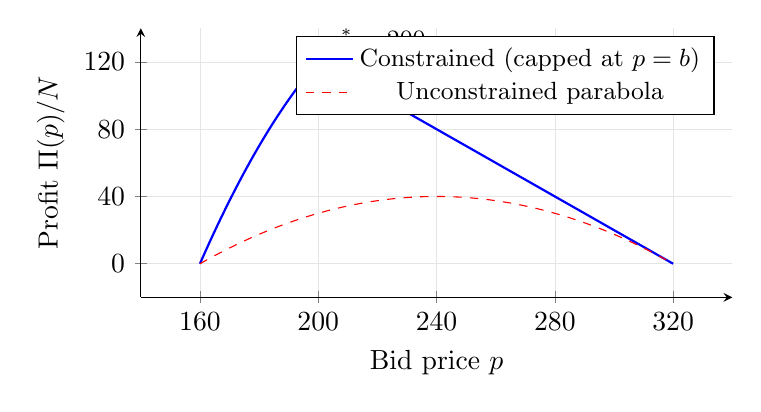
\begin{tikzpicture}
\begin{axis}[
  width=0.75\textwidth,
  height=5cm,
  xlabel={Bid price $p$},
  ylabel={Profit $\Pi(p)/N$},
  xmin=140, xmax=340,
  ymin=-20, ymax=140,
  xtick={160, 200, 240, 280, 320},
  ytick={0, 40, 80, 120},
  grid=both,
  grid style={line width=0.2pt, draw=gray!20},
  axis lines=left,
  legend pos=north east,
  legend style={font=\small},
]
% Unconstrained parabola for a=160, V=320: Pi = (p-160)/40 * (320-p) for p in [160,200]
% For p >= 200, Pi = 320 - p
\addplot[blue, thick, domain=160:200, samples=50]
  {(x-160)/40 * (320-x)};
\addplot[blue, thick, domain=200:320, samples=50]
  {320-x};
\addplot[red, dashed, domain=160:320, samples=50]
  {(x-160)*(320-x)/160};
\addplot[only marks, mark=*, mark size=2.5pt, blue] coordinates {(200, 120)};
\node[above right, font=\small] at (axis cs:200,120) {$p^*=200$};
\legend{Constrained (capped at $p=b$), , Unconstrained parabola}
\end{axis}
\end{tikzpicture}
\end{center}

\paragraph{Prosperity~3 numbers.}
Round~3, Part~1 \citep{frankfurtHedgehogs2025imcP3}:
$a = 160$, $b = 200$, $V = 320$, giving unconstrained $p^* = 240$.
But since $240 > b = 200$, the seller fraction saturates at~1
for $p \ge 200$, after which $\Pi(p) = N(320 - p)$ is decreasing.
So compare: $\Pi(200) = 120N$ versus $\Pi(240) = 80N$.  The
constrained optimum is $p^* = 200$, matching the Hedgehogs'
answer.

\subsection{Game-theoretic extension}

Part~2 added a competitive twist: reserves $\mathrm{Uniform}[250,
320]$, and profit was scaled down if your bid fell below the
population average~$\mu$:
\begin{equation}
  \Pi(p, \mu)
  \;=\;
  N \cdot \frac{p - 250}{70} \cdot (320 - p)
  \cdot \min\!\left(
    \left(\frac{320 - \mu}{320 - p}\right)^{\!3},\; 1
  \right).
  \label{eq:ch25_reserve_game}
\end{equation}
The cubic penalty punishes bids below average severely, creating
upward coordination pressure---every team wants to bid at or above
the average, pushing the average up.

\begin{intuitionbox}
This is adverse selection from \cref{ch:kyle_gm} in disguise.  A
Glosten--Milgrom market maker who quotes too generously is picked
off by informed traders; here, a team that bids below the crowd
average is ``picked off'' by the penalty.  Shade toward the
expected counterparty action.
\end{intuitionbox}

\paragraph{Equilibrium analysis.}
Without the penalty, the Part~2 optimum is $p^* = (320+250)/2 = 285$.
At a symmetric Nash, every team bids the same $\mu^*$ so the
penalty factor is~1, giving $\mu^* = 285$.

But the penalty is asymmetric: undershooting is punished cubically,
overshooting is not punished at all.  Teams that recognise this
shade above~$285$, which raises~$\mu$ and penalises those who did
not.  This ratchet pushes bids higher.

The Hedgehogs bid~$303$, anticipating overshoot.  The actual
average was~$287$---most teams did not model the twist---and they
overpaid by about $5.5\%$ versus the ex-post optimum
\citep{frankfurtHedgehogs2025imcP3}.

\begin{pitfallbox}[Over-correcting for the penalty]
This is a beauty contest: you bid on what others will bid on what
you will bid, \emph{ad infinitum}.  Sophisticated teams over-correct
(303 when the average is 287); naive teams anchor at 285 and drag
the average down.  When in doubt, shade toward the single-player
optimum, not toward infinity.
\end{pitfallbox}


%======================================================================
\section{Suitcase / Nash bargaining}
\label{sec:ch25_suitcases}
%======================================================================

Some manual rounds are cooperative bargaining: parties divide a
surplus, and the division depends on each side's outside option.
Prosperity ``suitcase'' rounds look like the container format
(\cref{sec:ch25_containers}) with a second pick at known cost, but
the underlying structure is Nash bargaining.

\subsection{Nash bargaining solution}

Two players $A$, $B$ bargain over a surplus~$S$.  If they agree,
$A$ gets $x$ and $B$ gets $S - x$; if not, they get disagreement
payoffs $d_A, d_B$.  Nash (1950) proved a unique division satisfies
four axioms (Pareto efficiency, symmetry, IIA, invariance to affine
utility transformations)---the one maximising the \emph{Nash product}:
\begin{equation}
  x^*
  \;=\;
  \arg\max_{x \;\in\; [d_A,\, S - d_B]}
  \;
  (x - d_A)(S - x - d_B).
  \label{eq:ch25_nash_bargaining}
\end{equation}

\begin{keyfactbox}[Nash bargaining solution]
For two players with disagreement payoffs $d_A$, $d_B$
dividing a surplus~$S$, the Nash bargaining solution is
\[
  x^*_A \;=\; d_A + \frac{S - d_A - d_B}{2},
  \qquad
  x^*_B \;=\; d_B + \frac{S - d_A - d_B}{2}.
\]
Each player gets their disagreement payoff plus half the net
surplus $S - d_A - d_B$.  Improving your outside option raises
your negotiated outcome one-for-one.
\end{keyfactbox}

\begin{proof}[Derivation]
Expanding the Nash product:
\[
  f(x) = (x - d_A)(S - x - d_B).
\]
This is a downward-opening parabola in~$x$.  Differentiating:
\[
  f'(x) = (S - x - d_B) - (x - d_A)
  = S - d_A - d_B - 2x.
\]
Setting $f'(x) = 0$ gives $x^* = (S - d_A - d_B + 2d_A)/2
= d_A + (S - d_A - d_B)/2$, confirming the formula.
\end{proof}

\subsection{Worked numerical example}

Two traders bargain over a bonus pool $S = 100{,}000$ with
disagreement payoffs $d_A = 20{,}000$ and $d_B = 30{,}000$, so
the net surplus is $50{,}000$.  Applying the formula:
\begin{align*}
  x^*_A &= 20{,}000 + \frac{50{,}000}{2}
  = 20{,}000 + 25{,}000 = 45{,}000, \\[4pt]
  x^*_B &= 30{,}000 + \frac{50{,}000}{2}
  = 30{,}000 + 25{,}000 = 55{,}000.
\end{align*}
Player~$B$'s stronger outside option ($d_B > d_A$) captures more
surplus.  If $A$ can improve to $d_A = 40{,}000$ (e.g.\ a competing
offer), the net surplus shrinks to $30{,}000$ and $A$'s allocation
rises to $55{,}000$---a $10{,}000$ gain from a $20{,}000$ improvement
in the outside option.

\subsection{Application to Prosperity container/suitcase rounds}

The Prosperity~3 Round~4 suitcase format mirrored Round~2's
containers but with a second pick at cost $25{,}000$
\citep{frankfurtHedgehogs2025imcP3}.  The Nash lens applies to
the second-pick decision: disagreement payoff is the single-pick
profit; the second-pick surplus must exceed its cost.

\paragraph{Second-pick decision rule.}
Take the second pick iff $E_2 > c$: with $E_2 = 40{,}000$ and
$c = 25{,}000$, net value is $+15{,}000$; with $E_2 = 20{,}000$
it is $-5{,}000$.  Since $E_2$ is an estimate, a close call near
$c$ is sensitive to error---decline when risk-averse.

\paragraph{Prosperity~3, Round~4 results.}
The Hedgehogs chose multipliers~37 and~50; their ranking was
60, 37, 50.  Actual crowd allocations differed substantially---%
multiplier~37 drew $4.79\%$ versus the predicted $2.09\%$---and
their combined $\approx 85{,}000$ SeaShells barely exceeded the
average of $82{,}000$ \citep{frankfurtHedgehogs2025imcP3}:

\medskip
\begin{center}
\begin{tabular}{c c c c c}
\toprule
\textbf{Mult.} & \textbf{Predicted $p_f$} & \textbf{Actual $p_f$} & \textbf{Pred.\ rank} & \textbf{Actual rank} \\
\midrule
60 & 4.25\% & 6.72\% & 1 & 8 \\
37 & 2.09\% & 4.79\% & 2 & 14 \\
50 & 2.98\% & 3.92\% & 3 & 6 \\
\bottomrule
\end{tabular}
\end{center}
\medskip

\begin{intuitionbox}
In the suitcase round, bargaining power against the crowd comes
entirely from predicting what others do.  A poor crowd model
means your ``outside option'' (naive-pick payout) dominates and
sophistication adds no edge---the Hedgehogs' Round~4 predictions
were off, and their profit barely exceeded average.
\end{intuitionbox}


%======================================================================
\section{News trading}
\label{sec:ch25_news_trading}
%======================================================================

The news-trading round presents products with current prices
plus news headlines hinting at future moves.  You size positions;
after the round, products settle at new prices and your profit
is the mark-to-market (position size times the realised price
move, i.e.\ the unrealised gain or loss valued at the final
quote).

\subsection{Bayesian updating framework}

Model product~$i$'s true percentage move as $\theta_i$; the
headline is a noisy signal~$s_i$.  Prior $\theta_i \sim
\Normal(\mu_0, \sigma_0^2)$ (often $\mu_0 = 0$ when agnostic).
For additive Gaussian noise $s_i = \theta_i + \varepsilon_i$,
$\varepsilon_i \sim \Normal(0, \sigma_\varepsilon^2)$, the
posterior is
\begin{equation}
  \theta_i \mid s_i
  \;\sim\;
  \Normal\!\left(
    \frac{\sigma_\varepsilon^2 \,\mu_0 +
          \sigma_0^2 \, s_i}
         {\sigma_0^2 + \sigma_\varepsilon^2},
    \;\;
    \frac{\sigma_0^2 \, \sigma_\varepsilon^2}
         {\sigma_0^2 + \sigma_\varepsilon^2}
  \right).
  \label{eq:ch25_bayesian_update}
\end{equation}
a precision-weighted average of prior and signal.

\begin{keyfactbox}[Bayesian posterior for Gaussian signal]
Given prior $\theta \sim \Normal(\mu_0, \sigma_0^2)$ and
signal $s = \theta + \varepsilon$ with
$\varepsilon \sim \Normal(0, \sigma_\varepsilon^2)$:
\[
  \E[\theta \mid s]
  \;=\;
  \underbrace{\frac{\sigma_\varepsilon^2}
    {\sigma_0^2 + \sigma_\varepsilon^2}}_{\text{weight on prior}}
  \mu_0
  \;+\;
  \underbrace{\frac{\sigma_0^2}
    {\sigma_0^2 + \sigma_\varepsilon^2}}_{\text{weight on signal}}
  s.
\]
As $\sigma_\varepsilon \to 0$ the posterior collapses to the
signal; as $\sigma_\varepsilon \to \infty$ it stays at the prior.
Same update rule as the Glosten--Milgrom dealer model
(\cref{ch:kyle_gm}).
\end{keyfactbox}

\subsection{Worked Bayesian example}

Product price $100$, prior $\theta \sim \Normal(0, 0.20^2)$
(no drift, $20\%$ volatility).  Headline gives signal $s = -0.35$
with noise $\sigma_\varepsilon = 0.25$.  Posterior mean:
\begin{align*}
  \E[\theta \mid s]
  &= \frac{\sigma_\varepsilon^2}{\sigma_0^2 + \sigma_\varepsilon^2}
  \cdot \mu_0
  + \frac{\sigma_0^2}{\sigma_0^2 + \sigma_\varepsilon^2} \cdot s \\
  &= \frac{0.0625}{0.04 + 0.0625} \cdot 0
  + \frac{0.04}{0.04 + 0.0625} \cdot (-0.35) \\
  &= 0 + \frac{0.04}{0.1025} \cdot (-0.35) \\
  &= 0.390 \times (-0.35)
  \;=\; -0.137.
\end{align*}
The posterior standard deviation is:
\[
  \hat{\sigma} = \sqrt{\frac{0.04 \times 0.0625}{0.1025}}
  = \sqrt{0.02439} \approx 0.156.
\]
Expect a $-13.7\%$ move with $15.6\%$ uncertainty.  The signal
pulled your view from $0\%$ toward $-35\%$ but only partway,
because the signal is noisy---a short with moderate conviction.

\subsection{Position sizing}

Given posterior mean $\hat{\theta}_i = \E[\theta_i \mid s_i]$
and variance $\hat{\sigma}_i^2$, Kelly (\cref{ch:kelly_risk})
sizes the bet.  With price~$P_i$ and lot limit~$L_i$, a
simplified Kelly-style allocation is:
\begin{equation}
  q_i
  \;=\;
  L_i \cdot \frac{\hat{\theta}_i}
  {\hat{\theta}_i^2 + \hat{\sigma}_i^2}
  \label{eq:ch25_kelly_news}
\end{equation}
with $q_i > 0$ buy, $q_i < 0$ sell: bet proportionally to edge
$\hat{\theta}_i$, scale down when $\hat{\sigma}_i^2$ is large.
In practice the position limits are small and direction matters
more than exact size.

\subsection{Worked example: Prosperity~3, Round~5}

Round~5 presented nine products with simulated news
\citep{frankfurtHedgehogs2025imcP3}.  The Hedgehogs estimated
directional moves and sized positions conservatively.  In the
table below, \textbf{Profit} is what they earned given their
actual bets, while \textbf{Optimal} is what a perfect oracle
knowing the actual move would have earned at the position
limit---the gap measures forecasting error, not sizing mistakes:

\medskip
\begin{center}
\small
\begin{tabular}{l r r r r}
\toprule
\textbf{Product} & \textbf{Est.\ move} & \textbf{Actual move} &
\textbf{Profit} & \textbf{Optimal} \\
\midrule
Haystacks       & $+12\%$ & $-0.48\%$ & $-3{,}240$  & $0$ \\
Ranch Sauce     & $+10\%$ & $-0.72\%$ & $-2{,}208$  & $0$ \\
Cacti Needle    & $-30\%$ & $-41.2\%$ & $32{,}160$  & $35{,}360$ \\
Solar Panels    & $-30\%$ & $-8.90\%$ & $-6{,}600$  & $1{,}640$ \\
Red Flags       & $+5\%$  & $+50.9\%$ & $9{,}700$   & $53{,}970$ \\
VR Monocle      & $+30\%$ & $+22.4\%$ & $9{,}600$   & $10{,}440$ \\
Quantum Coffee  & $-50\%$ & $-66.8\%$ & $87{,}339$  & $92{,}932$ \\
Moonshine       & $0\%$   & $+3.0\%$  & $0$         & $180$ \\
Striped Shirts  & $0\%$   & $+0.21\%$ & $0$         & $0$ \\
\midrule
\textbf{Total}  &         &           & $\mathbf{126{,}751}$ & $\mathbf{194{,}522}$ \\
\bottomrule
\end{tabular}
\end{center}
\medskip

\noindent
Biggest misses: Red Flags (+5\% vs.\ +50.9\%) and Solar Panels
(direction right, magnitude off).  Total profit captured $65\%$
of the theoretical optimum.

\begin{pitfallbox}[Overconfidence in signal precision]
The Hedgehogs anchored on Prosperity~1 and~2 analogies (e.g.\
assuming \texttt{Haystacks} behaved like a prior-year product).
This is prior anchoring: when the prior is strong and the signal
ambiguous, the update barely moves---but if the prior is wrong,
so is the posterior.  Defence: treat cross-year analogies as weak
priors (large $\sigma_0$) and let the signal dominate.
\end{pitfallbox}


%======================================================================
\section{Cross-cutting themes}
\label{sec:ch25_cross_cutting}
%======================================================================

Several threads run through all five manual-round archetypes.

\paragraph{EV is necessary but not sufficient.}
Every round reduces to an EV calculation, but its inputs---crowd
behaviour, signal precision, distributions---are uncertain.  The
skill is mental sensitivity analysis: how wrong can my inputs be
before the bet is $-$EV?

\paragraph{Game theory enters whenever the crowd matters.}
FX is pure optimisation (rates are given); containers and
reserve-price are games.  Diagnostic: if the payoff contains a
term indexed by others' actions, single-agent optimisation will
mislead you.

\paragraph{Bayesian updating is the meta-skill.}
News trading uses it explicitly; the container round uses it
implicitly (updating crowd-behaviour models from Round~2 to
Round~4 data).  On a trading floor it is the informal reflex
triggered by every new piece of information.

\begin{prosperitybox}
The Hedgehogs' manual strategy reveals a consistent philosophy:
\textbf{hedge against model error rather than maximise expected
profit} \citep{frankfurtHedgehogs2025imcP3}.

Round~1 (FX): brute-forced the optimum (rates deterministic, no
hedge needed).  Round~2 (containers): avoided the psychologically
salient multiplier~37 for a middle-of-the-road pick.  Round~3
(reserve price): over-bid to avoid the cubic penalty, accepting
a small loss.  Round~4 (suitcases): spread risk across two picks.
Round~5 (news): deliberately undersized positions.

Total manual PnL $\approx 252{,}000$ SeaShells across five rounds---%
well below the theoretical optimum, but with low variance and no
catastrophic round.  The lesson: \emph{when manual PnL is small
relative to algorithmic, play for safe EV, not maximum EV}.
\end{prosperitybox}


\begin{gsbox}
A Goldman trading desk tests the same skills: quick mental
arithmetic, Bayesian updating under time pressure, game-theoretic
positioning against counterparties.

When a client requests a price on a block of bonds, the trader
has seconds to: (i)~estimate fair value from the screen
(FX round-trip), (ii)~assess client information content
(Glosten--Milgrom, \cref{ch:kyle_gm}), (iii)~set bid--ask edge
(reserve-price problem), and (iv)~update the market view given
\emph{that client} calling \emph{now} (Bayesian news update).

A placement student who can explain the connection---``the
reserve-price round is client quoting with the cubic penalty
playing the role of adverse selection''---shows exactly the
structured thinking a desk head values.
\end{gsbox}


%======================================================================
\section{Key facts to memorise}
\label{sec:ch25_key_facts}
%======================================================================

\begin{enumerate}
  \item \textbf{FX triangular arbitrage:} compute the product of
  rates around a cycle.  If $>1$, the cycle is profitable.
  Enumerate all walks of length~$\le k$ to find the optimum.

  \item \textbf{Winner's curse:} in any auction or selection
  problem, the ``winner'' is the bidder with the most optimistic
  estimate.  Correct for this by modelling what others will do,
  not just what you would do alone.

  \item \textbf{Reserve-price optimum:} with uniform reserves
  on $[a, b]$ and resale value~$V$, the optimal bid is
  $p^* = (V + a)/2$, constrained to $[a, V]$.

  \item \textbf{Game-theoretic penalty:} when your payout depends
  on the crowd's average action, shade toward the crowd rather
  than toward the single-player optimum.  Over-correction is
  possible; the crowd is often less sophisticated than you fear.

  \item \textbf{Nash bargaining solution:} each party gets their
  disagreement payoff plus half the net surplus.  Improving your
  outside option improves your negotiated outcome one-for-one.

  \item \textbf{Bayesian updating for news:} posterior mean =
  precision-weighted average of prior and signal.  Noisy signals
  should move your view less.

  \item \textbf{Position sizing under uncertainty:} Kelly-style
  sizing says bet proportionally to expected edge, inversely to
  variance.  When uncertain, undersize.

  \item \textbf{Manual-round meta-strategy:} when manual PnL is
  small relative to algorithmic PnL, play for safe expected
  value, not maximum expected value.  Avoid catastrophic outcomes.
\end{enumerate}
